\documentclass[14pt]{extbook}
\usepackage{multicol, enumerate, enumitem, hyperref, color, soul, setspace, parskip, fancyhdr} %General Packages
\usepackage{amssymb, amsthm, amsmath, bbm, latexsym, units, mathtools} %Math Packages
\everymath{\displaystyle} %All math in Display Style
% Packages with additional options
\usepackage[headsep=0.5cm,headheight=12pt, left=1 in,right= 1 in,top= 1 in,bottom= 1 in]{geometry}
\usepackage[usenames,dvipsnames]{xcolor}
\usepackage{dashrule}  % Package to use the command below to create lines between items
\newcommand{\litem}[1]{\item#1\hspace*{-1cm}\rule{\textwidth}{0.4pt}}
\pagestyle{fancy}
\lhead{Progress Quiz 8}
\chead{}
\rhead{Version B}
\lfoot{4553-3922}
\cfoot{}
\rfoot{Fall 2020}
\begin{document}

\begin{enumerate}
\litem{
Determine the domain of the function below.\[ f(x) = \frac{3}{12x^{2} -32 x + 20} \]\begin{enumerate}[label=\Alph*.]
\item \( \text{All Real numbers except } x = a \text{ and } x = b, \text{ where } a \in [13.79, 15.39] \text{ and } b \in [15.86, 16.46] \)
\item \( \text{All Real numbers.} \)
\item \( \text{All Real numbers except } x = a, \text{ where } a \in [0.09, 1.33] \)
\item \( \text{All Real numbers except } x = a, \text{ where } a \in [13.79, 15.39] \)
\item \( \text{All Real numbers except } x = a \text{ and } x = b, \text{ where } a \in [0.09, 1.33] \text{ and } b \in [1.55, 1.9] \)

\end{enumerate} }
\litem{
Solve the rational equation below. Then, choose the interval(s) that the solution(s) belongs to.\[ \frac{-50}{-50x + 30} + 1 = \frac{-50}{-50x + 30} \]\begin{enumerate}[label=\Alph*.]
\item \( x_1 \in [-0.4, 1.6] \text{ and } x_2 \in [0.6,3.6] \)
\item \( \text{All solutions lead to invalid or complex values in the equation.} \)
\item \( x \in [-1.6,0.4] \)
\item \( x \in [0.6,1.6] \)
\item \( x_1 \in [-1.6, 0.4] \text{ and } x_2 \in [0.6,3.6] \)

\end{enumerate} }
\litem{
Solve the rational equation below. Then, choose the interval(s) that the solution(s) belongs to.\[ \frac{3x}{2x + 6} + \frac{-3x^{2}}{12x^{2} +50 x + 42} = \frac{3}{6x + 7} \]\begin{enumerate}[label=\Alph*.]
\item \( x_1 \in [0.04, 1.11] \text{ and } x_2 \in [-3.91,-1.76] \)
\item \( x_1 \in [0.04, 1.11] \text{ and } x_2 \in [-2.04,-1.39] \)
\item \( \text{All solutions lead to invalid or complex values in the equation.} \)
\item \( x \in [-1.62,-0.61] \)
\item \( x \in [-2.44,-1.5] \)

\end{enumerate} }
\litem{
Choose the graph of the equation below.\[ f(x) = \frac{1}{x - 1} - 1 \]\begin{enumerate}[label=\Alph*.]
\begin{multicols}{2}\item 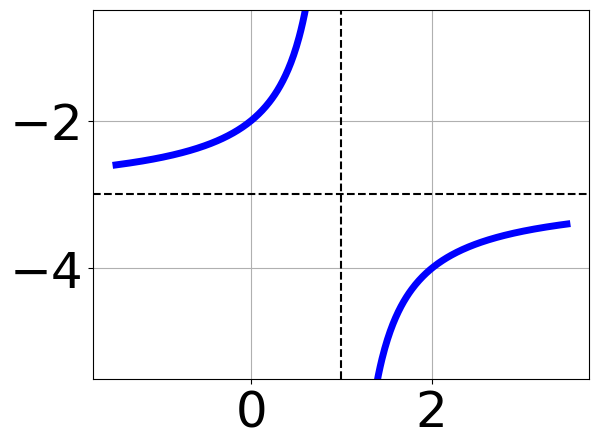
\includegraphics[width = 0.3\textwidth]{../Figures/rationalEquationToGraphCopyAB.png}\item 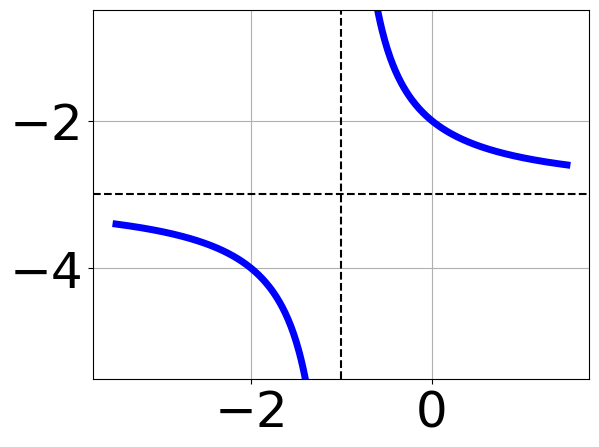
\includegraphics[width = 0.3\textwidth]{../Figures/rationalEquationToGraphCopyBB.png}\item 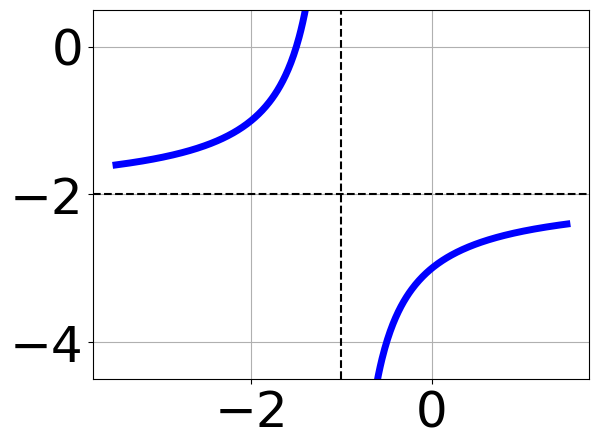
\includegraphics[width = 0.3\textwidth]{../Figures/rationalEquationToGraphCopyCB.png}\item 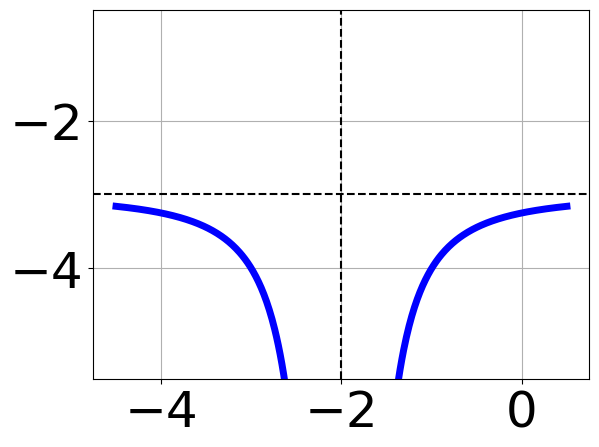
\includegraphics[width = 0.3\textwidth]{../Figures/rationalEquationToGraphCopyDB.png}\end{multicols}\item None of the above.
\end{enumerate} }
\litem{
Choose the equation of the function graphed below.
\begin{center}
    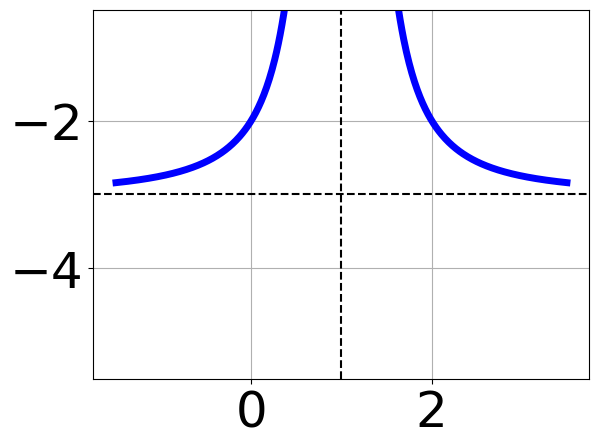
\includegraphics[width=0.5\textwidth]{../Figures/rationalGraphToEquationB.png}
\end{center}
\begin{enumerate}[label=\Alph*.]
\item \( f(x) = \frac{1}{(x - 1)^2} - 3 \)
\item \( f(x) = \frac{-1}{(x + 1)^2} - 3 \)
\item \( f(x) = \frac{-1}{x + 1} - 3 \)
\item \( f(x) = \frac{1}{x - 1} - 3 \)
\item \( \text{None of the above} \)

\end{enumerate} }
\litem{
Choose the graph of the equation below.\[ f(x) = \frac{1}{(x - 2)^2} + 1 \]\begin{enumerate}[label=\Alph*.]
\begin{multicols}{2}\item 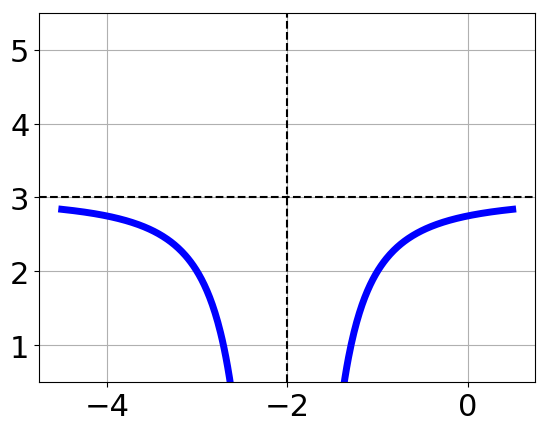
\includegraphics[width = 0.3\textwidth]{../Figures/rationalEquationToGraphAB.png}\item 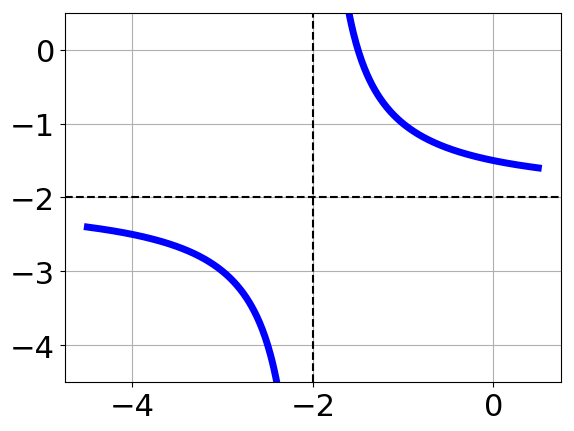
\includegraphics[width = 0.3\textwidth]{../Figures/rationalEquationToGraphBB.png}\item 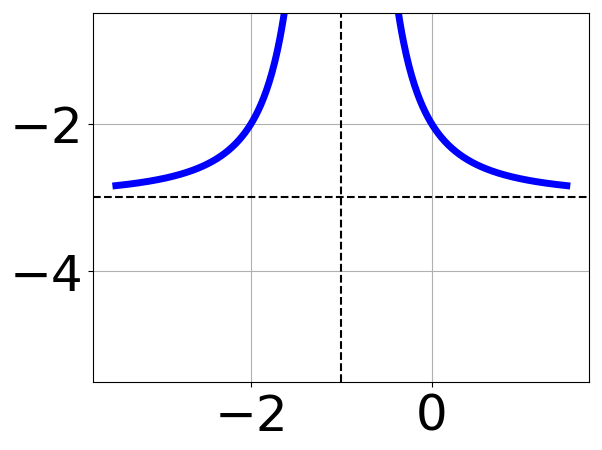
\includegraphics[width = 0.3\textwidth]{../Figures/rationalEquationToGraphCB.png}\item 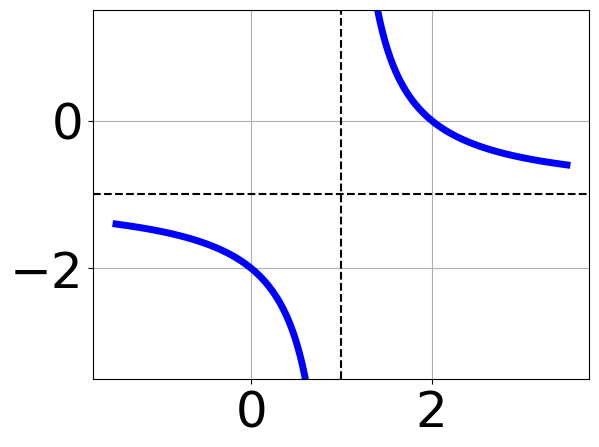
\includegraphics[width = 0.3\textwidth]{../Figures/rationalEquationToGraphDB.png}\end{multicols}\item None of the above.
\end{enumerate} }
\litem{
Solve the rational equation below. Then, choose the interval(s) that the solution(s) belongs to.\[ \frac{5x}{-7x -2} + \frac{-4x^{2}}{21x^{2} +34 x + 8} = \frac{6}{-3x -4} \]\begin{enumerate}[label=\Alph*.]
\item \( x \in [-1.7,-1.32] \)
\item \( x \in [1.21,2.75] \)
\item \( x_1 \in [-0.75, 0.03] \text{ and } x_2 \in [-0.2,4.1] \)
\item \( \text{All solutions lead to invalid or complex values in the equation.} \)
\item \( x_1 \in [-0.75, 0.03] \text{ and } x_2 \in [-2.5,0.7] \)

\end{enumerate} }
\litem{
Choose the equation of the function graphed below.
\begin{center}
    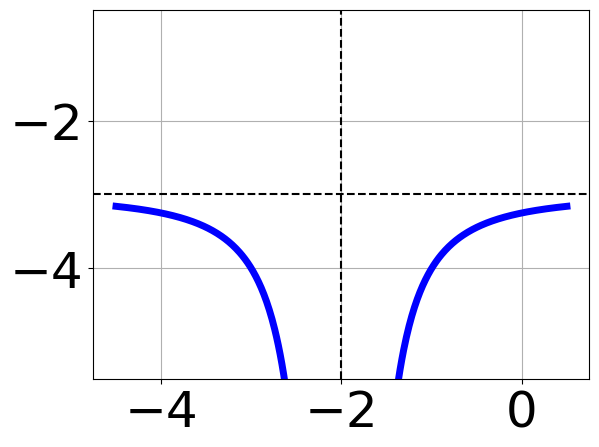
\includegraphics[width=0.5\textwidth]{../Figures/rationalGraphToEquationCopyB.png}
\end{center}
\begin{enumerate}[label=\Alph*.]
\item \( f(x) = \frac{-1}{x - 2} - 8 \)
\item \( f(x) = \frac{1}{x + 2} - 8 \)
\item \( f(x) = \frac{-1}{(x - 2)^2} - 8 \)
\item \( f(x) = \frac{1}{(x + 2)^2} - 8 \)
\item \( \text{None of the above} \)

\end{enumerate} }
\litem{
Determine the domain of the function below.\[ f(x) = \frac{6}{20x^{2} -49 x + 30} \]\begin{enumerate}[label=\Alph*.]
\item \( \text{All Real numbers.} \)
\item \( \text{All Real numbers except } x = a \text{ and } x = b, \text{ where } a \in [19.93, 20.12] \text{ and } b \in [29.94, 30.1] \)
\item \( \text{All Real numbers except } x = a \text{ and } x = b, \text{ where } a \in [1.17, 1.21] \text{ and } b \in [1.25, 1.36] \)
\item \( \text{All Real numbers except } x = a, \text{ where } a \in [19.93, 20.12] \)
\item \( \text{All Real numbers except } x = a, \text{ where } a \in [1.17, 1.21] \)

\end{enumerate} }
\litem{
Solve the rational equation below. Then, choose the interval(s) that the solution(s) belongs to.\[ \frac{4}{9x -6} + 2 = \frac{6}{-27x + 18} \]\begin{enumerate}[label=\Alph*.]
\item \( x \in [0.33,2.33] \)
\item \( \text{All solutions lead to invalid or complex values in the equation.} \)
\item \( x \in [-1,0] \)
\item \( x_1 \in [-1, 0] \text{ and } x_2 \in [-0.8,0.4] \)
\item \( x_1 \in [-0.67, 2.33] \text{ and } x_2 \in [0.7,2.2] \)

\end{enumerate} }
\end{enumerate}

\end{document}